\section{Introduction}

\subsection{Background}

Clustering is one of the most fundamental and extensively studied tasks in unsupervised learning---partitioning data points into subsets with high intra-group similarity and low inter-group similarity, without access to labels. Over decades of development, several canonical paradigms have emerged: prototype-based K-Means~\cite{macqueen1967}, density-based DBSCAN~\cite{ester1996}, graph-theoretic Spectral Clustering~\cite{ng2002}, and kernel-based Support Vector Clustering~\cite{benhur2001}. Each method exhibits distinct strengths on different geometric structures, with no universally optimal solution.

Support Vector Clustering (SVC)~\cite{benhur2001,benhur2000} is an important extension of kernel methods into unsupervised learning, with theoretical foundations in Support Vector Domain Description (SVDD)~\cite{tax1999,tax2004}. The core idea of SVC is to embed data through a nonlinear mapping $\phi: \mathbb{R}^d \rightarrow \mathcal{F}$ into a high-dimensional feature space $\mathcal{F}$, and then find the minimal hypersphere enclosing most data points in $\mathcal{F}$. Via the kernel trick, this hypersphere corresponds, in the original data space, to a set of nonlinear closed contour lines that tightly envelop the data distribution. By checking connectivity---verifying whether the line segment connecting two points remains entirely inside the hypersphere---SVC can capture cluster boundaries of arbitrary shape without prior assumptions about cluster geometry or count.

This theoretical elegance gives SVC natural advantages for non-convex structures such as half-moons and concentric circles. However, SVC's practical deployment faces a core bottleneck: the width parameter $q$ in the Gaussian kernel $K(x,y)=\exp(-q\|x-y\|^2)$ decisively influences clustering outcomes. The parameter $q$ controls the ``unfolding'' scale of data in feature space: too small a $q$ collapses the entire dataset into a single cluster; too large a $q$ isolates each point as its own cluster; only when $q$ falls within an appropriate interval can SVC produce meaningful partitions. This parameter sensitivity has been documented since~\cite{benhur2001}, yet has never been systematically resolved.

\subsection{Problem Statement}

Formally, given a dataset $X=\{x_1,\dots,x_N\}\subset\mathbb{R}^d$, SVC solves the dual Quadratic Programming (QP) problem:
\begin{equation}
\min_{\bm{\alpha}}\ \bm{\alpha}^T\mathbf{K}\bm{\alpha},\quad \text{s.t.}\ \sum_{i=1}^N\alpha_i=1,\ 0\leq\alpha_i\leq C \label{eq:svc_qp}
\end{equation}
where $K_{ij}=\exp(-q\|x_i-x_j\|^2)$ is the Gaussian kernel matrix and $C$ is the soft-margin penalty. Clustering quality depends jointly on two hyperparameters $(q,C)$. In unsupervised settings, selecting these parameters faces three fundamental difficulties:

\textbf{Difficulty~1: Non-differentiability.} Clustering performance as a function of $q$ lacks smooth derivatives---the ARI curve exhibits ``cliff-like'' jumps in parameter space (see Fig.~\ref{fig:q_effect}), rendering gradient-based optimization entirely ineffective.

\begin{figure}[t]
\centering
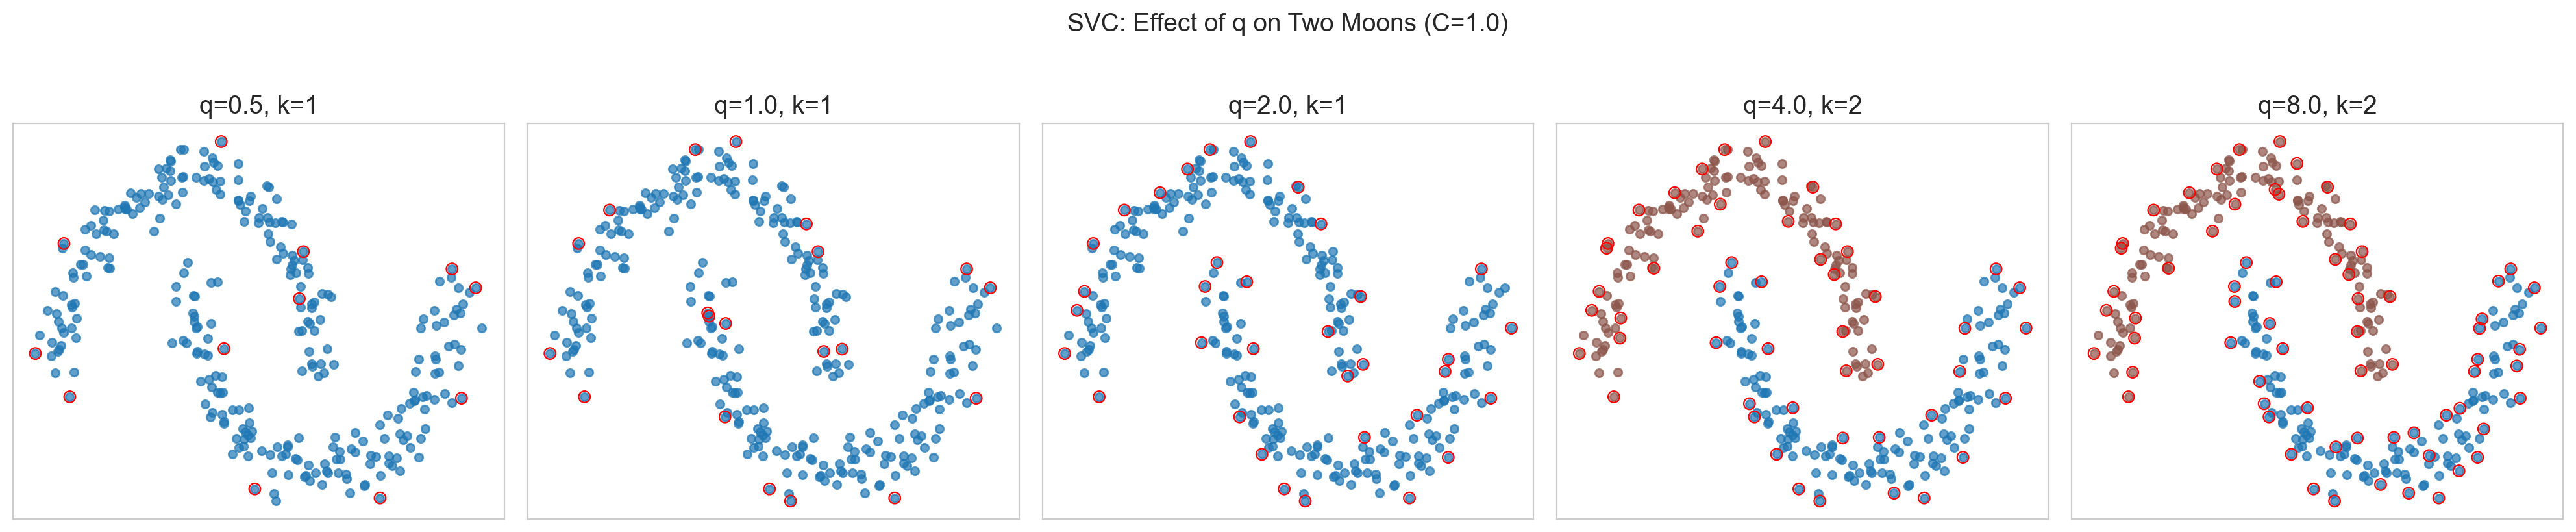
\includegraphics[width=\columnwidth]{fig/fig1_q_effect.png}
\caption{Parameter sensitivity of SVC on the Iris dataset (2D PCA). The ARI curve exhibits a ``cliff-like'' shape: a small shift in $q$ can cause the model to collapse from perfect clustering to complete failure. This non-differentiable behavior renders gradient-based optimization entirely ineffective.}
\label{fig:q_effect}
\end{figure}

\textbf{Difficulty~2: Unknowability.} Without labels, external metrics such as ARI are unavailable. Internal metrics (e.g., Silhouette coefficient, Davies-Bouldin index) are based on Euclidean distance measures that do not fully align with SVC's feature-space spherical geometry model and are therefore unreliable.

\textbf{Difficulty~3: Geometric dependence.} The optimal $q$ depends strongly on data geometry. In our experiments, $q^*\approx4.5$ for TwoMoons, $q^*\approx5.0$ for ConcentricCircles, yet SVC scores ARI~=~0 for OverlappingGaussians at \emph{any} $q$. No universal default exists.

\subsection{Contributions}

To address these challenges, we propose Adaptive Support Vector Clustering (ASVC), with the following core contributions:

\begin{enumerate}
\item \textbf{Automatic $q$-range estimation via local neighborhood statistics:} We use $k$-NN distances instead of global pairwise distances to estimate the kernel width search interval. The design motivation is that SVC's cluster boundaries are determined by local data structure, so $k$-NN distances that capture local scale are naturally more suitable than global distances as a statistical basis for $q$ estimation. A small $k$ value ($k=8$) reduces distance contamination from cross-cluster point pairs.

\item \textbf{Two-phase parameter search strategy:} The coarse phase uniformly samples on a logarithmic scale to achieve cross-order-of-magnitude coverage; the fine phase samples linearly around the coarse optimum for precision calibration, balancing search breadth with resolution.

\item \textbf{Continuous scoring function design:} A scoring function built from a cluster-count log-bonus, a support vector ratio Gaussian preference, and a piecewise BSV penalty forms a differentiable ``landscape'' in parameter space that guides the search toward high-quality solutions.

\item \textbf{Systematic experimental validation with dataset construction:} We benchmark comprehensively on six synthetic datasets with distinct geometric characteristics, including our specially constructed VaryingBlobs dataset (three Gaussian clusters with different variances) to verify ASVC's density-independent clustering capability.

\end{enumerate}
